\documentclass[10pt]{article}\usepackage[]{graphicx}\usepackage[]{color}
%% maxwidth is the original width if it is less than linewidth
%% otherwise use linewidth (to make sure the graphics do not exceed the margin)
\makeatletter
\def\maxwidth{ %
  \ifdim\Gin@nat@width>\linewidth
    \linewidth
  \else
    \Gin@nat@width
  \fi
}
\makeatother

\usepackage{Sweavel}


\usepackage{hyperref}
\usepackage{url}
\usepackage[a4paper]{geometry}
\usepackage{a4wide}
\usepackage{float}
\usepackage[english]{babel}
\usepackage[utf8]{inputenc}
\usepackage{csquotes}
\usepackage{amsmath}
\usepackage{amssymb}
\usepackage{xspace}
\usepackage[numbers]{natbib}
\bibliographystyle{unsrtnat}
\usepackage{subcaption}
\usepackage[font={small}]{caption}
\usepackage{booktabs}
\usepackage{listings}
\usepackage{cleveref}
\usepackage{lipsum}
\usepackage{graphicx}
\usepackage{epstopdf}
\graphicspath{{../figures/}}
\epstopdfsetup{outdir=./}
\newcommand{\approxtext}[1]{\ensuremath{\stackrel{\text{#1}}{=}}}
\newcommand{\matr}[1]{\mathbf{#1}}
\newcommand{\partt}[2]{\ensuremath{\dfrac{\partial {#1}}{\partial {#2}}}}
\renewcommand{\d}[1]{\ensuremath{\operatorname{d}\!{#1}}} % non-italized differentials
\newcommand{\h}[0]{\ensuremath{\hbar}} % hbar
\def\changemargin#1#2{\list{}{\rightmargin#2\leftmargin#1}\item[]}
\let\endchangemargin=\endlist 
\usepackage{amsthm}
\theoremstyle{plain}
\renewcommand{\theequation}{\thesection.\arabic{equation}}
\def\changemargin#1#2{\list{}{\rightmargin#2\leftmargin#1}\item[]}
\let\endchangemargin=\endlist    
\usepackage{xcolor}
\definecolor{Red}{rgb}{0.7,0,0}
\definecolor{Blue}{rgb}{0,0,0.8}
\usepackage{verbatim}
\def\changemargin#1#2{\list{}{\rightmargin#2\leftmargin#1}\item[]}
\let\endchangemargin=\endlist
\addtolength{\oddsidemargin}{-.35in}
\addtolength{\evensidemargin}{-.35in}
\addtolength{\textwidth}{.7in}
\usepackage{multicol}

% Stephen's stuff
\newcommand{\R}{\texttt{R}}
\newcommand{\Rfunction}[1]{{\texttt{#1}}}
\newcommand{\Robject}[1]{{\texttt{#1}}}
\newcommand{\Rpackage}[1]{{\mbox{\normalfont\textsf{#1}}}}
\usepackage{xcolor}
\definecolor{Red}{rgb}{0.7,0,0}
\definecolor{Blue}{rgb}{0,0,0.8}
\hypersetup{%
pdfusetitle,
bookmarks = {true},
bookmarksnumbered = {true},
bookmarksopen = {true},
bookmarksopenlevel = 2,
unicode = {true},
breaklinks = {false},
hyperindex = {true},
colorlinks = {true},
linktocpage = {true},
plainpages = {false},
linkcolor = {Blue},
citecolor = {Blue},
urlcolor = {Red},
pdfstartview = {Fit},
pdfpagemode = {UseOutlines},
pdfview = {XYZ null null null}
}
%% Listings
\lstset{ 
language=R,                     % the language of the code
basicstyle=\footnotesize,       % the size of the fonts that are used for the code
numbers=left,                   % where to put the line-numbers
numberstyle=\tiny\color{gray},  % the style that is used for the line-numbers
stepnumber=1,                   % the step between two line-numbers. If it's 1, each line will be numbered
numbersep=5pt,                  % how far the line-numbers are from the code
backgroundcolor=\color{white},  % choose the background color. You must add \usepackage{color}
showspaces=false,               % show spaces adding particular underscores
showstringspaces=false,         % underline spaces within strings
showtabs=false,                 % show tabs within strings adding particular underscores
rulecolor=\color{black},        % if not set, the frame-color may be changed on line-breaks within not-black text (e.g. commens (green here))
tabsize=2,                      % sets default tabsize to 2 spaces
captionpos=b,                   % sets the caption-position to bottom
breaklines=true,                % sets automatic line breaking
breakatwhitespace=false,        % sets if automatic breaks should only happen at whitespace
title=\lstname,                 % show the filename of files included with \lstinputlisting;
% also try caption instead of title
keywordstyle=\color{Blue},      % keyword style
commentstyle=\color{orange},    % comment style
stringstyle=\color{Red},        % string literal style
escapeinside={\%*}{*)},         % if you want to add a comment within your code
morekeywords={*,...}            % if you want to add more keywords to the set
} 

\epstopdfDeclareGraphicsRule{.tga}{png}{.png}{%
  convert #1 \OutputFile
}
\AppendGraphicsExtensions{.tga}

%%% Document specific
\newcommand{\course}{Structural Biology}
\newcommand{\ass}{1}
\newcommand{\term}{Lent term 2017}
%\bibliography{pga1}

%%% Title page
\title{
  \bf \course: Assignment \ass \\[1em]
  \small{University of Cambridge}
}

\author{Henrik Åhl}
\date{\today}
\renewcommand{\textfraction}{0.05}
\renewcommand{\topfraction}{0.8}
\renewcommand{\bottomfraction}{0.8}
\renewcommand{\floatpagefraction}{0.75}
\newcommand{\CA}{C$_\alpha$\xspace}



%%% Actual document
\begin{document}
\date{\today}
\maketitle
\setcounter{page}{1}


% \date{\today}
\maketitle
% \begin{abstract}
% 	{\bf 
% 		%\begin{changemargin}{-.8cm}{-.8cm}
% 		This is an abstract abstract.
% 	}
% \end{abstract}

\begin{multicols*}{2}
	\section*{Preface}
	This is an assignment report in connection to the \textit{\course}
	module in the Computational Biology course at the University of Cambridge,
	\term. All related code is as of \date{\today} available through a
	Github repository by contacting \href{mailto:hpa22@cam.ac.uk}{hpa22@cam.ac.uk}.
	\subsection*{Part A}
	\paragraph*{i}
	Inspecting the unbound structure as assigned, we find a molecular complex consisting of principally two anti-parallel beta-sheets (one of three strands, one of 6) wrapping around to form a tubular shape. The beta-sheets are connected through intermediate carbon-dominated strands, holding the structure together. A very small helix is also inferred in the data, as can be seen as in blue in \cref{fig:unbound_cartoon} and \cref{fig:unbound_VDW} in \emph{NewCartoon} and \emph{VDW} visualisation format respectively. Both figures are also aligned in order to show the capture cavity of the molecule, as is easist seen in \cref{fig:unbound_cartoon}. The backbone on one of the ends of the protein also appears to be open in such a way that it appears to possibly utilise this end to interact and attach to the larger Toll-like receptor complex. In contrast, the other end appears more stable, with more inferred closed circuits. 
		  
	Over the course of the trajectory, the molecule also appears to be quite flexible with respect to its subdomains, with the cavity opening in particular seeming quite variable. When the water molecules are also accounted for, we can note that no such molecules appear to be present within the ligand cavity, which might be because of polar repulsion and an intractable free energy landscape. However, due to the insufficient resolution to analyse this, we are unable to draw any decisive conclusions.
		
	\begin{figure}[H]
		\centering
		\includegraphics[trim={2cm 2.5cm 3cm 5cm}, clip, width=.4\textwidth]{unbound_cartoon}
		% \includegraphics{../figures/prot1_topview}
		\caption{Unbound protein at $t=0$ in the \emph{NewCartoon} visual theme. The capturing cavity is present foremost in this figure.}
		\label{fig:unbound_cartoon}
	\end{figure}
	
	\begin{figure}[H]
		\centering
		\includegraphics[trim={2cm 2cm 1cm 3cm}, clip, width=.4\textwidth]{unbound_VDW}
		\caption{Same as above, but in the \emph{VDW} theme, giving a more realistic estimate of the atoms' electrostatic surfaces.}
		\label{fig:unbound_VDW}
	\end{figure}
		
	\paragraph*{ii, iii}
	Simulating the protein from its initial state, it is clear that the binding cavity quickly closes off, making it seemingly inaccessible from the outside without prior interaction. The protein then resumes in this state over the course of the simulation, with mostly its tube-end backbone strands moving about significantly; especially the end containing the helix conformation appears visually particularly variable. Also the backbone on the backside of the protein as seen from when observing the cavity is highly variable. 
	
	Indeed, looking at the protein aligned to its initial state over the whole trajectory confirms the above mentioned observations. \Cref{fig:unbound_startvsend} shows a comparison between the initial (blue) and final state (red) of the protein in the simulation trajectory. In particular, movement in the part connecting to the helix, as well as the capturing cavity are particularly noticeable. 
		
	\paragraph*{iv}
	\begin{figure}[H]
		\centering
		\includegraphics[width=.4\textwidth]{unbound_aligned_startvsend.tga}
		\caption{Comparison between the structure at the initial (blue) and final (red) conformation. Note in particular how the cavity has closed.}
		\label{fig:unbound_startvsend}
	\end{figure}
	
	Observing the various parts of the molecule, and their general movement produces figure \cref{fig:trajs}. We find that the majority of the variability is attributed to movement of the backbone, which is mainly goverend by movement of the beta sheets. Due to the helix being small in comparison to the rest of the molecule, its contribution to the overall variability is minor, which in particular can be seen when the summed RMSD of the beta-sheets and the helix is plotted. This put further insight into the above mentioned observation in that the helix itself is not very variable, but rather the backbone connected to it.
		
\begin{Schunk}
\begin{figure}[H]

{\centering 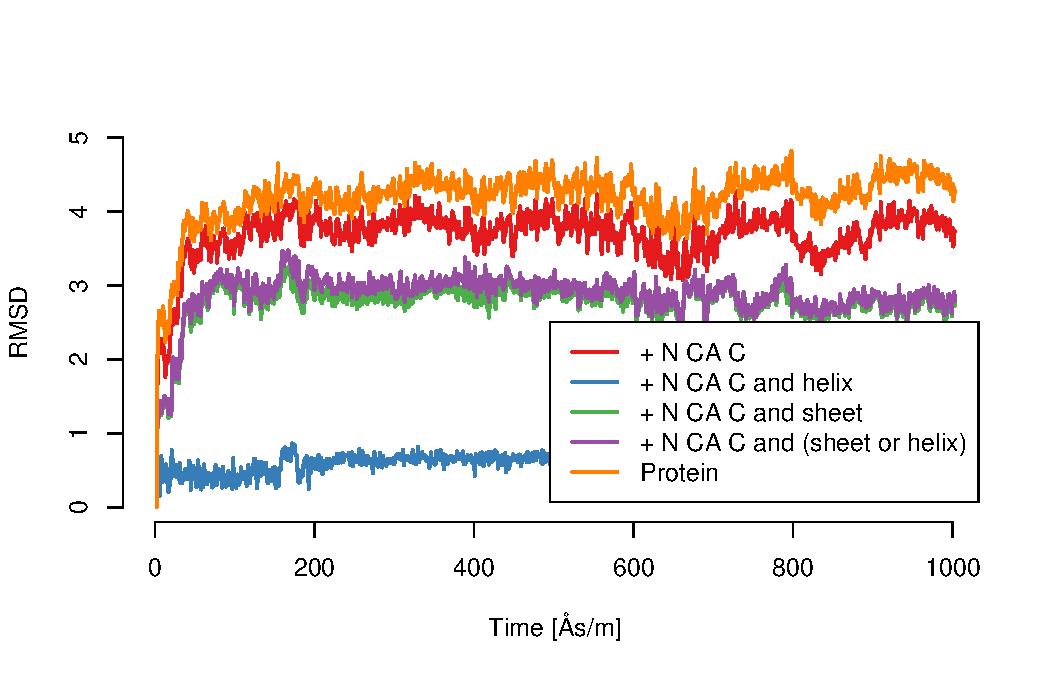
\includegraphics[width=\maxwidth]{figure/twocolumn-trajs-1} 

}

\caption[Spatial variations for select parts of the protein over the simulation]{Spatial variations for select parts of the protein over the simulation. Notably, the protein as a whole changes significantly in its conformation, which is mainly driven by movement of the major structures, such as the beta-sheets and the overall backbone.}\label{fig:trajs}
\end{figure}
\end{Schunk}
	
	\paragraph*{v}
	The Ramachandran plot for time $t = 0$ in \cref{fig:rama} shows the $\phi$ and $\psi$ angles for all the residues in the protein. Narrowing down the analysis, the beta sheet residues all have their data points located in the upper left corner, whereas the helix is located in the middle-left one. In other words, the important residues are all located in energetically allowed regions. Nevertheless, when accounting for the whole protein, some residues are indeed located outside of these, as the figure shows. At the end of the simulation, some clustering towards the coloured regions has occured, although many residues are still part of an incorrect conformation; most of these being C$_\alpha$ atoms. Disregarding these faulty conformations, the \CA atoms are otherwise spread out among the three islands, and continue to be so as the simulation progresses.
	
	\begin{figure}[H]
		\centering
		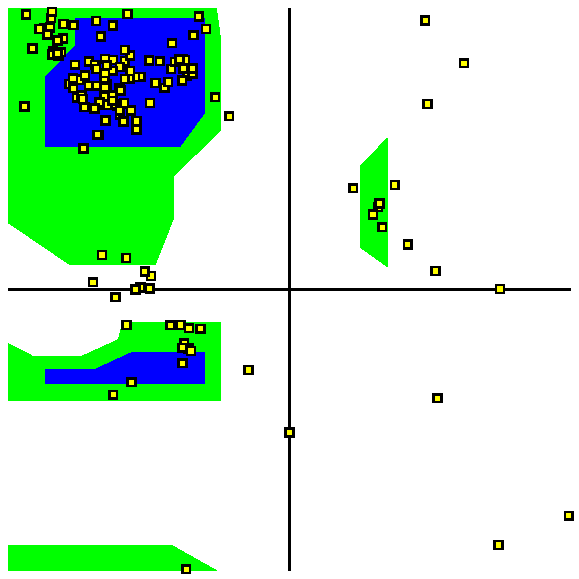
\includegraphics[width=.3\textwidth]{ramaplot.pdf}
		\caption{Ramachandran plot at $t = 0$, showing a clustering of the residues in the allowed energy conformations. However, some residues occur outside of these, and stay or get exchanged throughout the simulation.}
		\label{fig:rama}
	\end{figure}
	
\end{multicols*}
\paragraph*{vi, vii}
\begin{figure}[H]
	\centering
	\includegraphics[trim={2cm 1.6cm 0 0}, clip, width = \textwidth]{../figures/timeline}
	\caption{Structural inference on the residues in the system, with colour signifying inferred secondary structure. Most beta-sheets remain very stable throughout, with variations mostly in the edgemost parts of the conformation. Some regions are more variable than others, e.g.\ the ALA107 residue, which likely is such because of its unshielded position on the protein.}
	\label{fig:timeline}
\end{figure}
\begin{multicols*}{2}
	In the Timeline view, we see how the domains change over time for the different residues. As is to be expected from having observed the full trajectory, the beta sheets are fairly stable, with the varying parts being the edgemost ones. Similarly, the parts involved in forming the helix domain are likewise very variable. We also see the formation of new, pink domains. In general, most domains are stable overall, but most residues also alternate into some other domain at some point. \Cref{fig:domchange} shows a midway alteration in domains under the trajectory. Note in particular the occurence of a new, pink loop.like domain up top.
		
	\begin{figure}[H]
		\centering
		\includegraphics[trim={9cm 8cm 9cm 6cm}, clip, width = .3\textwidth]{../figures/domainchange_snapshot}
		\caption{Snapshot during simulation of change in inferred domains. Note in particular the occurence of a new, pink, loop-like domain near the top of the complex.}
		\label{fig:domchange}
	\end{figure}
	
	\paragraph*{viii}
\begin{Schunk}
\begin{figure}[H]

{\centering 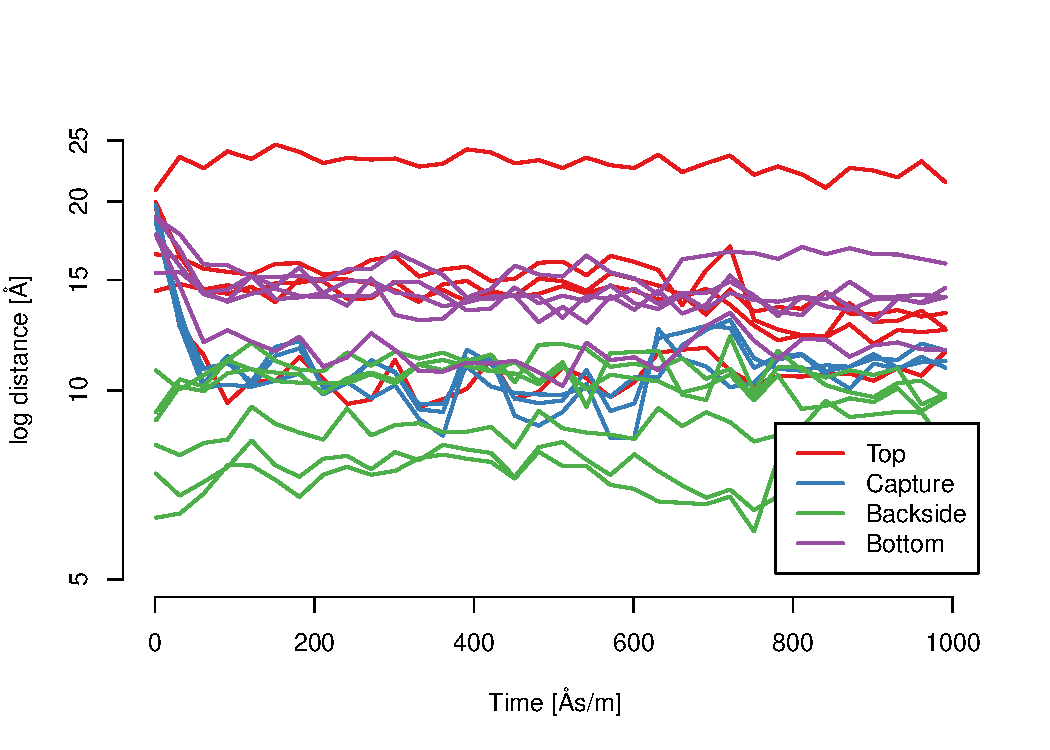
\includegraphics[width=\maxwidth]{figure/twocolumn-dists-1} 

}

\caption[Analysis in change in distance of four select parts of the protein]{Analysis in change in distance of four select parts of the protein. Here 'top' denotes the end of the protein which has an inferred 'open' backbone, i.e. with unconnected backbone loops. It can clearly be seen that the capture gap is the one strucutural part of the protein which changes significantly in the initial stages of the simulation.}\label{fig:dists}
\end{figure}
\end{Schunk}
		
		
	Analysis of the variability in distance between certain molecules is visible in \cref{fig:dists}, where the logarithmic distance for the distances beteween select atoms is given. Note in particular how the one part of the protein which changes in variability is the capturing cavity, because of the enclosing of the capture. In addition, we see how the topmost part, which we identify as the end of the tube with an open backbone, is contantly very variable, as we also see visually.
		
	% PLOT FIGURE OF THE THREE REGIONS HERE. 
	\paragraph*{ix}
  \Cref{fig:charged} shows the charged molecules overlaid on the inferred structure of the protein. Noticeably, most charged compounds are located far away from the backbone, as well as from each other. Similarly, the polar amino acids are all located in the outmost parts of the protein (\cref{fig:unbound_polar}). The more flexible parts of the protein also tend to consist of smaller amino acids (not shown).
		
		Interestingly, the protein consists of to a large extent of hydrophobic amino acids ({\cref{fig:hydroandali,fig:unbound_all_hydrophobic}}. This suggests that incoming lipids will bind with their tails inside the cavity, as the hydrophilic head would be comparatively inclined to be aligned outwards. The hydrophobic amino acids are also fairly evenly spread out across the cavity, with only minor gaps.
		
  \begin{figure}[H]
		\centering
		\includegraphics[trim={2cm 3cm 5.5cm 5cm}, clip, width = .45\textwidth]{../figures/charged}
		\caption{Charged residues overlaid on the \emph{NewCartoon} template of the molecule. Most of these are situated on the outsides of the protein, and not close to the cavity.}
		\label{fig:charged}
	\end{figure}

	\begin{figure}[H]
		\centering
		\includegraphics[trim={4cm 2.5cm 5cm 4.5cm}, clip, width = .45\textwidth]{../figures/unbound_polar}
		\caption{Likewise, the polar amino acids are like the encapsulating group located primarily on the outermost parts. }
		\label{fig:unbound_polar}
	\end{figure}
	
	  \begin{figure}[H]
		\centering
		\includegraphics[trim={5cm 4cm 7cm 5.5cm}, clip, width = .45\textwidth]{../figures/unbound_hydrophobicandaliphatic}
		\caption{Hydrophobic and aliphatic amino acids.}
		\label{fig:hydroandali}
	\end{figure}
	
  \begin{figure}[H]
		\centering
		\includegraphics[trim={2cm 2.5cm 5cm 4.5cm}, clip, width = .45\textwidth]{../figures/unbound_all_hydrophobic}
		\caption{All hydrophobic amino acids. These are fairly evenly spread out across the protein and also present within the cavity.}
		\label{fig:unbound_all_hydrophobic}
	\end{figure}
		
		
	\paragraph*{x} 
	In the beginning of the simulation, a few water molecules are present inside the cavity, whereas later on no such molecules are enclosed (see earlier remarks). Throughout the timecourse, the water molecules appear to interact with the structure mainly through its hydrogen, and appears to otherwise be evenly spread out across the whole protein.
		
	\paragraph*{xi}
The molecule turns around one of its axes, initially being positioned with its functional ring being positioned inside of the cavity. At the end of the simulation, however, the residue has been pushed out of the cavity and effectively turned ca 180$^\circ$ such that the aromatic ring is on the outside of the complex.

\section*{Part B}
	\paragraph*{i-iv}
  We first note that with the ligand bound, there is no inferred alpha helix domain anymore. Compared to the unbound protein, the Ramachandran plot for the bound counterpart tells of a similar distribution of residues with the same angles.
  
Identifying changes in distances for the protein's vital parts (\cref{fig:bounddists}), i.e. the front- and backend of the cavity, we see that there are no significant changes in distances over the whole timecourse, likely because the structure is already close to its functional energy minimum. Also, just as we can expect, the functional parts, i.e.\ the parts involved in the capture process are the most variable, whereas the backside of the protein is fairly stable throughout. In addition, the beta sheets are more stable than the outermost parts of the cavity.
  
\begin{Schunk}
\begin{figure}[H]

{\centering 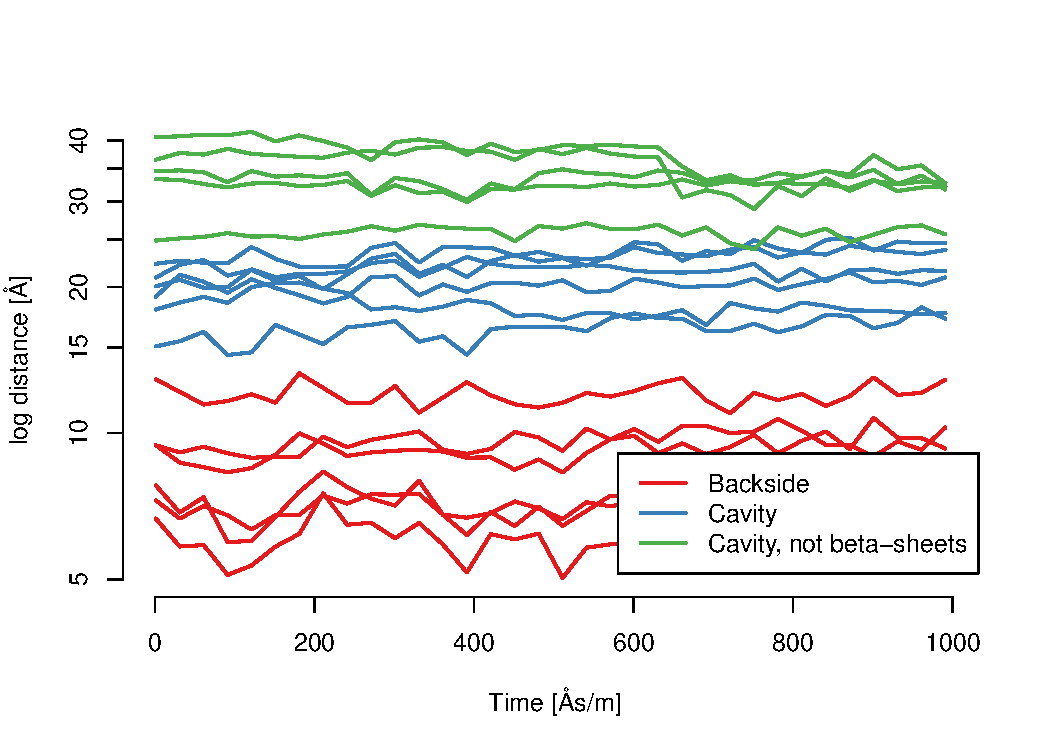
\includegraphics[width=\maxwidth]{figure/twocolumn-bounddists-1} 

}

\caption[Analsysis of the distance between atoms on either end of the labelled structures]{Analsysis of the distance between atoms on either end of the labelled structures. As expected, the backside of the protein is the most stable, whereas the beta-sheets are affiliated with larger movements.}\label{fig:bounddists}
\end{figure}
\end{Schunk}

Doing the same for the ligand itself, measuring distances between atoms on the heads and tails respectively, it is easily seen that the tail parts are significantly more volatile than the heads, showing signs of reorganisation within the cavity throughout the simulation. In contrast, distances between atoms on the heads stay surprisingly stable, which ought to be because the stabilising bonds they are connected to each other with, and which the five tails encapsulated in the cavity lack. 

\begin{Schunk}
\begin{figure}[H]

{\centering 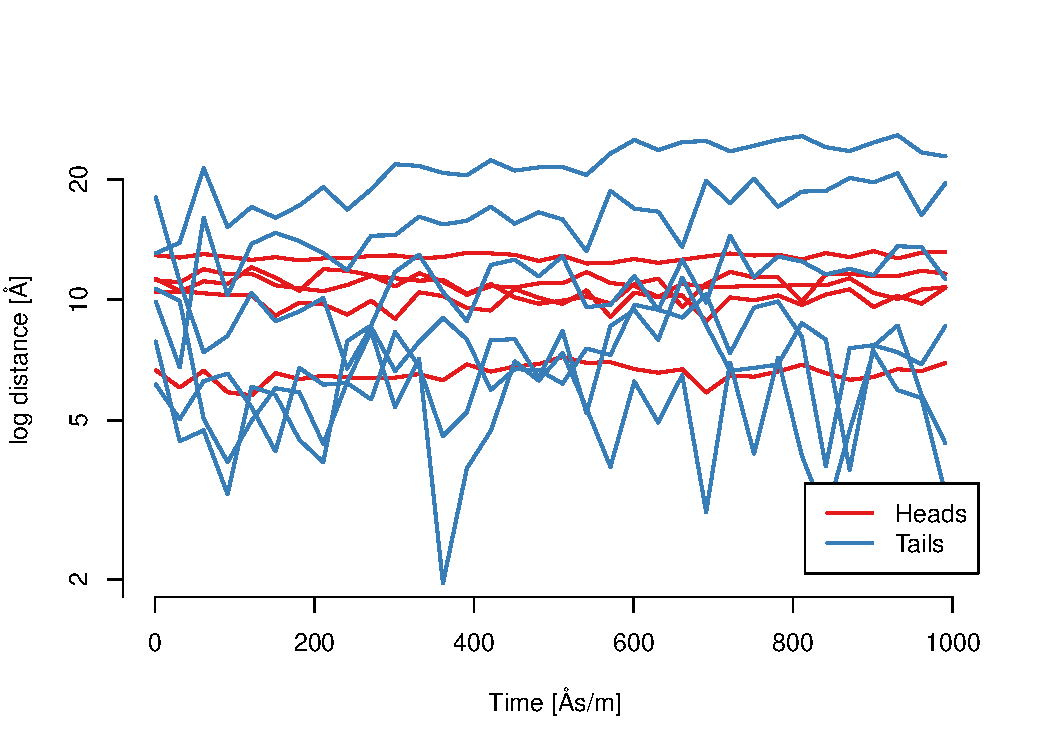
\includegraphics[width=\maxwidth]{figure/twocolumn-liganddists-1} 

}

\caption[Distances between select atoms on a few structurally interesting parts of the protein]{Distances between select atoms on a few structurally interesting parts of the protein. The headgroups are clearly much more stable than the tails, possibly due to electrostatic interactions with aminoacids involved in locking in the }\label{fig:liganddists}
\end{figure}
\end{Schunk}

The only positive amino acid binding to a phosphate group which we are able to identify is a sole arginine, which binds to phosphate group one of the ligand, as seen in \cref{fig:phosphatebinding}. However, also an aspartate and a glutamic acid, which are both negative, bind to the two phosphate groups through intermediate Na ions, which therefore indeed bridge the interaction. We also observe (not shown) that basic residues form contacts primarily with neutral ones and aliphatic ones. 

	\begin{figure}[H]
		\centering
		\includegraphics[trim={2cm 2.5cm 5cm 4.5cm}, clip, width = .45\textwidth]{../figures/bound_positive_aa_bindstoligandP1}
		\caption{Positive amino acids within 5 Ångström of the ligand. Snapshot taken at the very end of the simulation. Only a single ARG is present. However, when also including negative amino acids, which are intuitively less likely to interact with the negatively charged headgroups, we find that these bind to the phosphate groups via intermediate Na ions (not shown).}
		\label{fig:phosphatebinding}
	\end{figure}  
	
	Interestingly, in order to bind the ligand, the bound complex appear to be more flexible with respect to the non-sheet surfaces, indicating that the ligand intercedes with the ordinary path of least resistance, which ends up being what effectively entangles it in the cavity. Withing the cavity, the hydrophobic residues in the protein creates a hospitable environment, and does along with locking of the polar headgroups keep ligand in place. 
	
	In the non-bound states, the protein visually appears more rigid with respect to the overall structure, whereas it in the bound case has to adapt to the incoming ligand. In other words, the trajectory in the bound case is more varied, due to the induced environmental change. However, at the point where the ligand has stabilised somewhat, the other structure appears more variable; especially the helix moves away a bit at some of the later timepoints. 
	
\end{multicols*}
	\paragraph*{v}
	  \begin{figure}[t]
		\centering
		\includegraphics[width = .7\textwidth]{../figures/wholeprot}
		\caption{TLR4 associated with the MD2 protein, with residue Phe126 shown in red, aligned inwards to the protein.}
		\label{fig:wholeprot}
	\end{figure}
\begin{multicols*}{2}
In \cref{fig:wholeprot} the protein associated with the rest of the complex can be seen, with Phe126 coloured in red. Reminiscing the earlier observations of Phe126 turning during activation, it appears possible that the conformational change accompanied with the residue inhibits the protein when set free, but that this effect is hampered when the ligand is bound. However, if the ligand is smaller, e.g.\ due to fewer tails or similar, the change will still be able to occur to some extent, thus inhibiting TLR4. This would explain the observed decay in pronounciation for ligands with fewer tails. 
	
\bibliography{references}
\end{multicols*}
\end{document}
